
    Heterogeneous accelerators often disappoint.
    They provide the prospect of great performance, but only deliver it when
    using vendor specific optimized libraries or domain specific languages.
    This requires considerable legacy code modifications, hindering the adoption
    of heterogeneous computing.

    This paper develops a novel approach to automatically detect opportunities
    for accelerator exploitation.
    We focus on calculations that are well supported by established APIs: sparse
    and dense linear algebra, stencil codes and generalized reductions and
    histograms.
    We call them {\em idioms} and use a custom constraint-based Idiom
    Description Language (IDL) to discover them within user code.
    Detected idioms are then mapped to BLAS libraries, cuSPARSE and clSPARSE and
    two DSLs: Halide and Lift.

    We implemented the approach in LLVM and evaluated it on the NAS and Parboil
    sequential C/C++ benchmarks, where we detect 60 idiom instances.
    In those cases where idioms are a significant part of the sequential
    execution time, we generate code that achieves 1.26$\times$ to over
    20$\times$ speedup on integrated and external GPUs.

\section{Introduction}

    Heterogeneous accelerators provide the potential for great performance.
    However, achieving that potential is difficult.
    General purpose languages such as OpenCL \cite{nvidia11guide} provide
    portability, but the achieved performance often disappoints
    \cite{lee09openmp}.
    This shortfall has led vendors to deliver specialized libraries to bridge
    the gap \cite{clblas}.  Alternatively, domain specific languages (DSLs)
    \cite{Franchetti09OL,Rompf:2012:LMS:2184319.2184345} have been proposed,
    attempting to deliver  both portability and performance
    \cite{Ragan-Kelley2013Halide}.

    Hardware becomes increasingly heterogeneous, ({\it e.g.} TPU
    \cite{jouppi2017datacenter}).
    This means library or DSL based programming is likely to become far more
    common and future programmers are expected to target those APIs.

    However, there are problems with this trend.
    Firstly, users have to learn multiple specialized DSLs and vendor-specific
    libraries.
    Secondly, users have to restructure and rewrite their applications to use
    them.
    Having to learn and understand several new APIs and then rewrite existing
    applications is a severe impediment to the wide-spread efficient
    exploitation of heterogeneous hardware.
    Ideally, we would like a mechanism that automatically maps existing code to
    heterogeneous hardware using the appropriate APIs without user effort.

    Our approach is based on detecting specific structures or {\em idioms} in
    user code that correspond to the functionality of existing APIs for
    heterogeneous acceleration.
    We focus on idioms that are well supported by existing libraries and DSLs.
    These are likely to be both relevant to existing code bases and have
    efficient heterogeneous implementations.
    We consider sparse and dense linear algebra, stencils and generalized
    reductions and histograms.

    At the heart of our approach is the ability to describe each idiom in a
    concise Idiom Description Language (IDL).
    After the user's C/C++ program has been compiled down to LLVM IR, our tool
    reads in an IDL program and translates into a set of constraints.
    These are passed to a fast solver to search the user's program, detecting
    all idiom instances.

    Once detected, the idioms are mechanically translated into the appropriate
    DSL or replaced with a library call.
    This optimized code is then linked into the original program.
    We currently target the libraries cuSparse, clSparse, cuBLAS, clBLAS for
    sparse and dense linear algebra and target the DSL Halide
    \cite{Ragan-Kelley2013Halide} for stencil computations.
    We also target Lift \cite{SteuwerRD17} - a data parallel language that
    supports generalized reductions as well as stencils and linear algebra.
    This allows the freedom to target many APIs for the same idiom and pick the
    implementation that best suits the target platform. 

    New idioms can be easily added thanks to the flexibility of IDL.
    This provides a powerful means of determining whether a new heterogeneous
    API matches existing code without touching the core compiler.
    The idioms addressed in this paper can be expressed in less than 500 lines
    of IDL code.
    Our approach is also highly robust, it has been applied to the entire NAS
    and Parboil benchmark suites and is evaluated on three platforms.

    We present a novel approach that:
    \begin{itemize}
    \item Defines a programming language for specifying code idioms, the Idiom
          Description Language (IDL)\\[-.9em]
    \item Implements common idioms in IDL to automatically discover
          opportunities for accelerator exploitation\\[-.9em]
    \item Efficiently translates and maps the detected idioms to APIs for
          heterogeneous systems
    \end{itemize}

    While there has been much research in
    using constraints for program analysis~\cite{nielson2015principles},
    there is little prior work in its use for idiom
    detection. In \cite{ginsbach2017discovery}, constraints are used for
    detecting reductions, but this is tightly coupled to a specialized code
    generation phase for small-scale multi-core systems.

    The work most similar in approach concerns discovery of stencil computation
    and mapping to the Halide DSL.
    Helium \cite{Mendis2015Helium} recovers stencils from image-processing
    binaries.
    This requires large scale dynamic analysis of binary traces and replacing
    them with Halide calls. 
    This is significantly extended in~\cite{Kamil2016Verified} which detects
    stencils in FORTRAN.
    In this work the focus is on inferring post invariants based on syntax
    guided synthesis in translation to Halide.
    However, it uses a narrow approach to selecting code snippets and relies on
    well structured FORTRAN with occasional user annotations.
    Our approach is distinct in that we use an external  programming language to
    describe the idioms we are interested in.
    This allows an unbounded set of idioms  to be considered across arbitrary
    programs and is not restricted to stencils. 

    To summarize, this paper presents an automatic approach that discovers
    idioms in legacy code and maps them to heterogeneous platforms via
    libraries and DSLs.
    We apply it to 21 C/C++ programs from the NAS and Parboil benchmark suites
    and demonstrate that it detects more reductions, stencils, matrix
    multiplications and sparse matrix-vector computations than existing schemes.
    For the idioms that dominate execution time, we generate code and evaluate
    on 3 platforms: a multi-core CPU, an integrated and an external GPU. Overall
    we detect 60 idioms.
    In 10 programs these dominate sequential execution time and are worth
    exploiting.
    This results in speedups ranging from 1.26$\times$ to over 20$\times$.

\section{Overview}

    Our approach is automatic and has been implemented inside the LLVM compiler
    infrastructure.
    It takes arbitrary sequential C/C++ programs as input.
    Using the clang compiler, the input source code is compiled into a Single
    Static Assignment (SSA) intermediate representation.
    We then search this representation for particular idioms which are replaced
    with calls to specific APIs.
    Finally, the code generated by the LLVM compiler and the output of the idiom
    specific code generators/libraries are linked together into a binary,
    producing an optimized program.
    LLVM was chosen as it is the best supported SSA-based compiler;
    the methodology could easily be transferred to other infrastructures such as
    gcc.

\subsection{Compiler Flow}

    The structure of our approach is described in more detail in
    \autoref{fig:methodology}.
    Our compiler takes two programs as inputs: the first is the user's program
    source code, the second describes the idioms we wish to detect using our
    idiom description language (section 3).
    The same idioms, of course, can be detected across many user programs, so
    the IDL program does not have to change from one run to the next.

\begin{figure}[t]
    \centering
    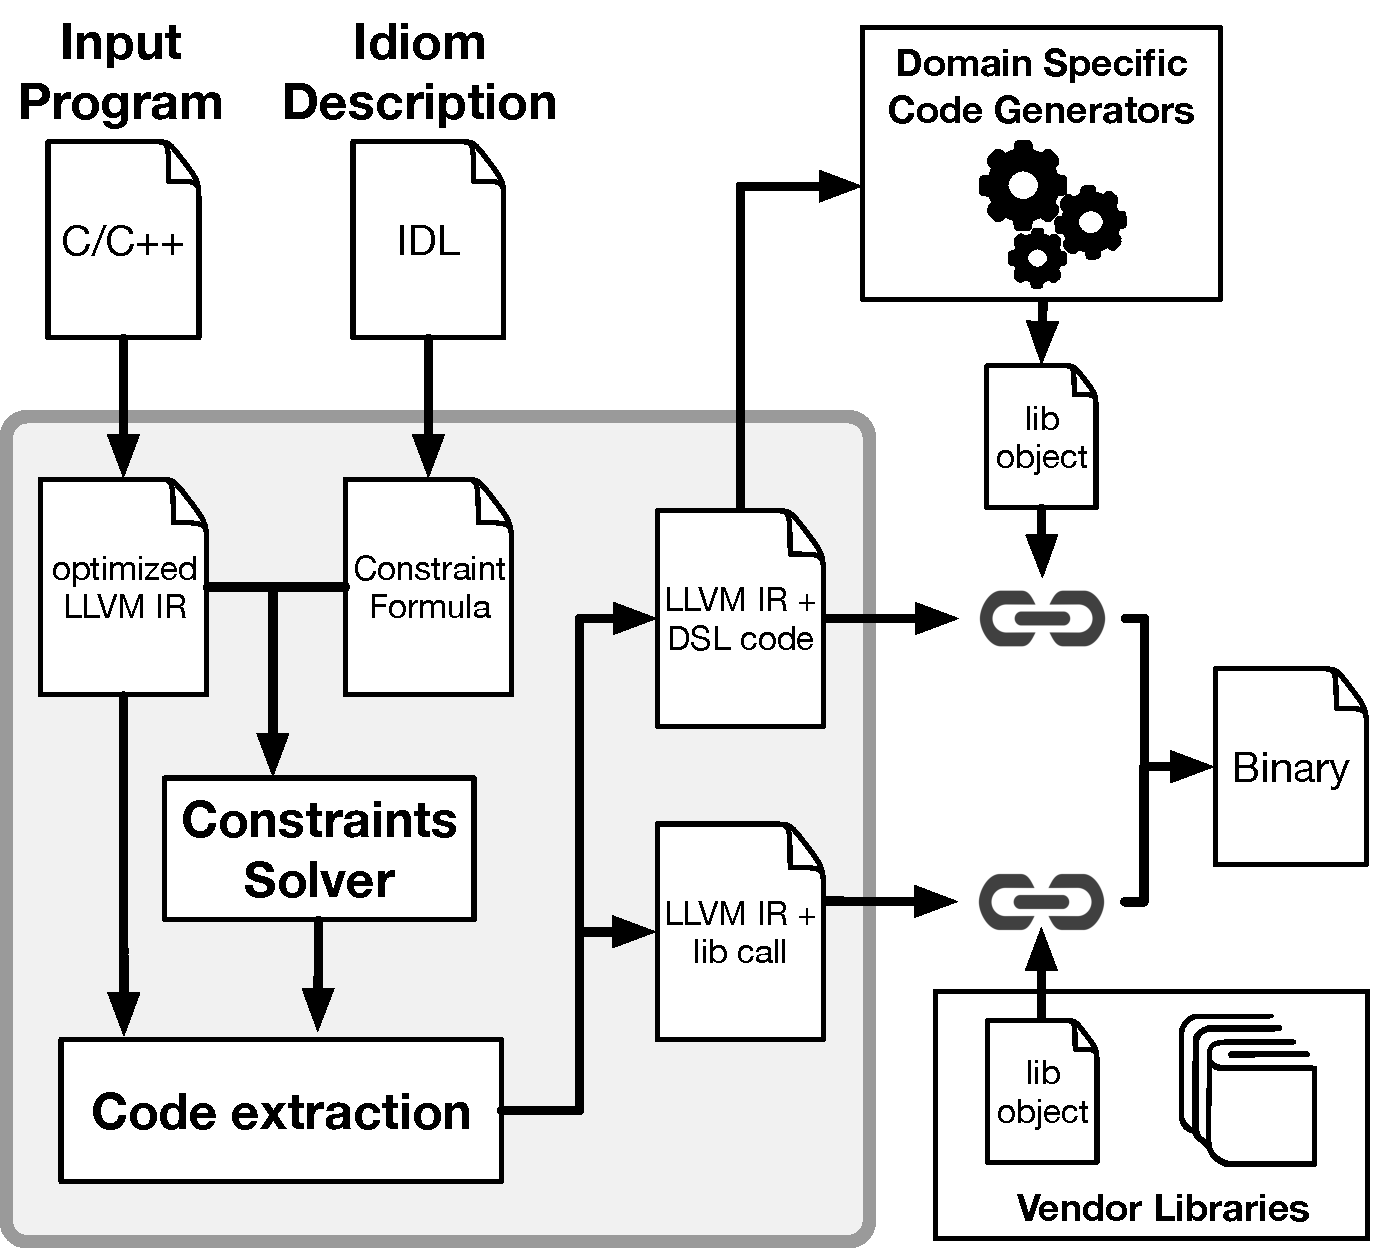
\includegraphics[width=\linewidth]{figures/compiler_flow.pdf}
    \caption{Workflow of our system}
    \label{fig:methodology}
    \vspace{-0.5em}
\end{figure}

    The program source code is compiled to optimized LLVM IR code  while the
    idiom description is translated into constraints and represented
    internally as a C++ object.
    The C++ representation of the constraints and the user program LLVM IR code
    are then passed as inputs to a backtracking solver
    \cite{ginsbach2017discovery}, which detects all cases where the idioms can
    be found in the LLVR IR.

    The recognized idioms as well as the LLVM IR code are then passed on
    to the transformation phase of our system.  The sections of code that
    correspond to computational idioms are extracted and reformulated for
    the appropriate heterogeneous APIs.  For library  APIs this means replacing
    the code covered by the idiom with a library call. 
    For domain specific language interfaces,
    things are a little more involved. As before, we first extract the code
    associated with the idiom and replace it with a function call. This
    extracted code is now translated into the appropriate DSL and then
    passed on to the external DSL compiler which optimizes and generates
    code. The generated code is then linked
    with the object code from the main program.

    Determining the best heterogeneous APIs to use for a given platform
    and the best idioms to exploit will become a major issue as the number
    of idioms and APIs grows.  Currently, in this paper, we just try all
    applicable libraries and DSLs and pick the best executing
    code. Determining the best option is future work.

\subsection{IDL Example}

    At the core of our approach is IDL, which is described in \autoref{sec:idl}.
    A fundamental part of its design is the
    ability to detect  complex idioms.  Here we first focus on a simple example
    to show how IDL works.  Consider the standard factorizing
    optimization that applies the algebraic rule of distributivity
    \[(x*y)+(x*z) = x*(y+z)\]
    to simplify calculations by reducing the number of multiplications in an
    expression.
    The established way of implementing such an optimization is to hard code a
    detection compiler pass.
    In LLVM, this is 47 lines of code inside the \texttt{instcombine} pass.

\begin{figure}[t]
\begin{lstlisting}[language={constraints},escapechar=|,basicstyle=\linespread{1.133}\scriptsize\ttfamily]
Constraint FactorizationOpportunity
( {sum} is add instruction and
  {left_addend} is first argument of {sum} and
  {left_addend} is mul instruction and
  {right_addend} is second augment of {sum} and
  {right_addend} is mul instruction and
  |\label{line:factorFirstLeft}|( {factor} is first argument of {left_addend} or
  |\label{line:factorSecondLeft}|  {factor} is second argument of {left_addend}) and
  |\label{line:factorFirstRight}|( {factor} is first argument of {right_addend} or
  |\label{line:factorSecondRight}|  {factor} is second argument of {right_addend}))
End
\end{lstlisting}
\vspace{-0.3cm}
\caption{IDL formulation of (x*y)+(x*z) pattern}
\label{fig:IDLfactorization}
\end{figure}

Using IDL,  we can formulate this in only a few lines of an easily understandable program (\autoref{fig:IDLfactorization}).
For this simple example, the underlying constraint problem is immediately visible: There are four variables
\texttt{sum}, \texttt{left\_addend}, \texttt{right\_addend}, \texttt{factor} and nine individual constraints
that are combined with boolean operators.

\pagebreak

From the formulation in \autoref{fig:IDLfactorization}, the IDL compiler builds a representation of the underlying constraint problem that is passed to a constraint solver.
For a given section of user code, this solver returns the set of factorization opportunities, each containing four entries
\texttt{sum}, \texttt{left\_addend}, \texttt{right\_addend}, \texttt{factor} that refer to values inside the user code.
\autoref{fig:firstexample} shows a simple example.
The incoming C code is translated to optimized LLVM IR.
The solver then finds a single solution to the constraint problem.

\begin{figure}[h]
Original C code:
\begin{lstlisting}[basicstyle=\footnotesize\ttfamily]
int example(int a, int b, int c) {
    int d = a;
    return (a*b) + (c*d);
}
\end{lstlisting}
\vspace{1em}
Resulting LLVM IR:
\begin{lstlisting}[escapeinside={(*}{*)},language={LLVM},basicstyle=\footnotesize\ttfamily]
define i32 @example(i32 %a, i32 %b, i32 %c) {
  %1 = mul i32 %a, %b
  %2 = mul i32 %c, %a
  %3 = add i32 %1, %2
  ret i32 %3
}
\end{lstlisting}
\vspace{1em}
Detected factorization opportunities:
\begin{lstlisting}[escapeinside={(*}{*)},language={},basicstyle=\footnotesize\ttfamily]
{ "sum" :          %3,
  "left_addend" :  %1,
  "right_addend" : %2,
  "factor" :       %a }
\end{lstlisting}
\vspace{-0.3cm}
\caption{Demonstration of simple idiom detection}
\label{fig:firstexample}
\end{figure}

In this case, the variable {\tt sum} is matched to the value {\tt \%3}, an add instruction, while the variables {\tt left\_addend} and {\tt right\_addend} match the left and right operands {\tt \%1} and {\tt \%2} of this instruction. 

Lines \autoref{line:factorFirstLeft} and \autoref{line:factorSecondLeft} of \autoref{fig:IDLfactorization} say that {\tt factor} can either be the first argument OR the second argument of {\tt left\_addend}.
As the {\tt left\_addend} is {\tt \%1}, then {\tt factor} can be either {\tt \%a} or {\tt \%b}.
Similarly lines \autoref{line:factorFirstRight} and \autoref{line:factorSecondRight} of \autoref{fig:IDLfactorization} say that {\tt factor} can be be the first argument OR the second argument of the {\tt right\_addend}.
As the {\tt right\_addend} is {\tt \%1}, then {\tt factor} can be either {\tt \%c} or {\tt \%a}.
The two disjunctions in Lines 7-10 are connected by AND, so they must both hold.
\begin{equation}
\begin{split}
((factor = a) \lor & (factor = b)) \\\land ((factor = c) \lor & (factor = a)) \\
\implies & factor = a 
\end{split}
\nonumber
\end{equation}
The only value of {\tt factor} that satisfies this condition is {\tt factor = \%a}.
Therefore, the solution at the bottom of \autoref{fig:firstexample} is the only factorization opportunity in the code.

\begin{figure}[p]
    \begin{lstlisting}[language=MyCpp, basicstyle=\linespread{0.75}\small\ttfamily]
for (j = 0; j < ([{\bf m}]); j++) {
  d = 0.0;
  for (k = ([{\bf rowstr }])[j]; k < ([{\bf rowstr}])[j+1]; k++)
    d = d + ([{\bf a}])[k]*([{\bf z}])[([{\bf colidx}])[k]];
  ([{\bf r}])[j] = d; }
\end{lstlisting}
\vspace{-4.4mm}
\begin{lstlisting}[language={LLVM}, basicstyle=\linespread{0.75}\tiny\ttfamily,
                   label={fig:spmvexample1}, caption={Sparse linear algebra in C and LLVM IR}]
; <label>:2:
  %j = phi i64 [ %j_next, %12 ], [ 0, %1 ]
  %j_cond = icmp slt i64 %j, ([{\bf \%m}])
  br i1 %j_cond, label %3, label %13([\vspace{1mm}])
; <label>:3:
%4 = getelementptr i32, i32* ([{\bf \%rowstr}]), i64 %j
  %5 = load i32, i32* %4
  %j_next = add nuw nsw i64 %j, 1
  %6 = getelementptr i32, i32* ([{\bf \%rowstr}]), i64 %j_next
  %7 = load i32, i32* %6
  %k_begin = sext i32 %5 to i64
  %k_end = sext i32 %7 to i64
  br label %8([\vspace{1mm}])
; <label>:8:
  %k = phi i64 [ %k_next, %9 ], [ %k_begin, %dnext ]
  %d = phi double [ 0.0, %3 ], [ %d_next, %9 ]
  %k_cond = icmp slt i64 %iv, %k_end
  br i1 %k_cond, label %9, label %12([\vspace{1mm}])
; <label>:9:
  %a_addr = getelementptr double, double* ([{\bf \%a}]), i64 %k
  %a_load = load double, double* %a_addr
  %cix_addr = getelementptr i32, i32* ([{\bf \%colidx}]), i64 %k
  %cix_load = load i32, i32* %cix_addr
  %10 = sext i32 %cix_load to i64
  %z_addr = getelementptr double, double* ([{\bf \%z}]), i64 %10
  %z_load = load double, double* %z_addr
  %11 = fmul double %a_load, %z_load
  %d_next = fadd double %d, %11
  %k_next = add nsw i64 %k, 1
  br label %8([\vspace{1mm}])
; <label>:12:
  %r_addr = getelementptr double, double* ([{\bf \%r}]), i64 %j
  store double %d, double* %r_addr
  br label %2
\end{lstlisting}
\vspace{-0.287cm}
%\end{figure}

\centering
\vspace{0.0em}
{\centering
\begin{minipage}{0.05\linewidth}
\vspace{0pt}
\centering
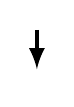
\begin{tikzpicture}[ultra thick]
 \draw [black,   -latex      ] (0,0.5) -- (0,0) node [] {};
\end{tikzpicture}
\end{minipage}
\begin{minipage}{\linewidth}
% \vspace{-5pt}
\centering
\textbf{Idiom detection with IDL program in \Cref{fig:spmv}}
\end{minipage}
\begin{minipage}{0.05\linewidth}
\vspace{0pt}
\centering
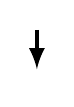
\begin{tikzpicture}[ultra thick]
 \draw [black,   -latex      ] (0,0.5) -- (0,0) node [] {};
\end{tikzpicture}
\end{minipage}
}

%\begin{figure}
{\centering
\footnotesize 
\begin{tabular}{l|l}
\textbf{Variable Name} & \textbf{Assigned IR Value}\\
\hline
iterator                    & \texttt{\%j}\\
inner.iter\_begin           & \texttt{\%k\_begin}\\
inner.iter\_end             & \texttt{\%k\_end}\\
inner.iterator              & \texttt{\%k}\\
idx\_read.value             & \texttt{\%cix\_load}\\
indir\_read.value           & \texttt{\%a\_load}\\
seq\_read.value             & \texttt{\%z}\\
\end{tabular}
\hspace{0.5cm}
\begin{tabular}{l|l}
\textbf{Variable Name} & \textbf{Assigned IR Value}\\
\hline
output.address              & \texttt{\%r\_addr}\\
iter\_begin                 & \texttt{0}\\
iter\_end                   & \texttt{\%\bf m}\\
idx\_read.base\_pointer     & \texttt{\%\bf colidx}\\
seq\_read.base\_pointer     & \texttt{\%\bf a}\\
indir\_read.base\_pointer   & \texttt{\%\bf z}\\
\dots                       & \dots\vspace{-0.5mm}\\
\end{tabular}

}

\caption{Constraint solution for sparse mv}
\label{fig:spmvexample2}
%\end{figure}

\centering
\vspace{0.0em}
{\centering
\begin{minipage}{0.05\linewidth}
\vspace{0pt}
\centering
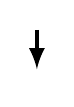
\begin{tikzpicture}[ultra thick]
 \draw [black,   -latex      ] (0,0.5) -- (0,0) node [] {};
\end{tikzpicture}
\end{minipage}
\begin{minipage}{\linewidth}
% \vspace{-5pt}
\centering
\textbf{Code generation: insert arguments, replace code}
\end{minipage}
\begin{minipage}{0.05\linewidth}
\vspace{0pt}
\centering
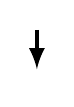
\begin{tikzpicture}[ultra thick]
 \draw [black,   -latex      ] (0,0.5) -- (0,0) node [] {};
\end{tikzpicture}
\end{minipage}
}


%\begin{figure}
\begin{lstlisting}[language=C, basicstyle=\linespread{0.75}\small\ttfamily,
                   label={fig:spmvexample3}, caption={Generated function call to cuSPARSE}]
cusparseDcsrmv(context,
    CUSPARSE_OPERATION_NON_TRANSPOSE, ([{\bf m}]), n,
    ([{\bf rowstr}])[([{\bf m}])+1]-([{\bf rowstr}])[0], &gpu_1, descr, gpu_([{\bf a}]),
    gpu_([{\bf rowstr}]), gpu_([{\bf colidx}]), gpu_([{\bf z}]), &gpu_0, gpu_([{\bf r}]));
\end{lstlisting}
\vspace{-0.287cm}
\end{figure}

\subsection{Sparse Linear Algebra in IDL}

    Although the previous example illustrated how constraints can be applied to 
    program analysis, we want to detect much more complex idioms and 
    map them to existing APIs.

    The C code in \autoref{fig:spmvexample1} shows the performance bottleneck of
    the NAS \emph{Conjugate Gradient (GC)} benchmark, as well as the
    corresponding LLVM IR code.
    It implements a standard operation from sparse linear algebra, namely a
    multiplication of a sparse matrix in Compressed Sparse Row (CSR) format with
    a dense vector.

    This code contains several features that make it unsuitable for most
    established compiler optimizations:
    The iteration domain of the nested loop is memory dependent (line 3) and
    there is indirect memory access (line 4).
    This makes the iteration domain of the loop nest non-polyhedral and the
    access structure to memory non-affine.
    Under these conditions, simple data dependence models, but also
    sophisticated analysis based on the polyhedral model, would fail.

    We can express this idiom in IDL (\autoref{sec:idioms}, \autoref{fig:spmv}).
    The IR code, together with the IDL program, is fed into a constraint solver,
    which outputs a constraint solution as shown in \autoref{fig:spmvexample2}.
    We can see that different parts of the IR have been assigned to IDL
    variables.

    \autoref{fig:spmvexample3} shows how this solution is used to generate a
    call to a cuSPARSE procedure.
    The solution variables are inserted into the {\tt cusparseDcsrmv} code
    template as function arguments. 
    The original code is then cut out and replaced with this function call.
    The cuSPARSE library is then linked with the object code produced by the
    LLVM compiler, resulting in a speedup of $17\times$ on a GPU as described in
    \autoref{sec:results}.

    Central to our approach is the ability to detect idioms.
    In the next section we introduce a powerful description language that is
    capable of expressing a wide class of idioms that are suitable for
    acceleration by heterogeneous hardware.

\section{Idiom Description Language}

\begin{figure*}[t]
    \begin{minipage}{15cm}
\small
\begin{align*}
\text{spec\text{if}ication} ::= {}&\text{\bf Constraint}\ \left<\text{\bf s}\right>\ \left<\text{constraint}\right>\ \text{\bf End}\\[-1pt]
\text{constraint} ::= {}&\left<\text{\text{atomic}}\right> \mid \left<\text{grouping}\right> \mid \left<\text{\text{collect}}\right> \mid \left<\text{\text{rename}}\right> \mid \left<\text{\text{rebase}}\right> \mid \text{\bf `('}\ \left<\text{constraint}\right>\ \text{\bf `)'}\\[-1pt]
\text{grouping} ::= {}&\left<\text{conjunction}\right> \mid \left<\text{disjunction}\right> \mid \left<\text{inheritance}\right> \mid \left<\text{forall}\right> \mid \left<\text{forsome}\right> \mid \left<\text{forone}\right> \mid \left<\text{if}\right>\\[-1pt]
\text{conjunction} ::= {}&\text{\bf `('}\ \left<\text{constraint}\right>\ \text{\bf and}\ \left<\text{constraint}\right>\ \left\{ \text{\bf and}\ \left<\text{constraint}\right> \right\}\ \text{\bf `)'}\\[-1pt]
\text{disjunction} ::= {}&\text{\bf `('}\ \left<\text{constraint}\right>\ \text{\bf or}\ \left<\text{constraint}\right>\ \left\{ \text{\bf or}\ \left<\text{constraint}\right> \right\}\ \text{\bf `)'}\\[-1pt]
\text{inheritance} ::= {}&\text{\bf inherits}\ \left<\text{\bf s}\right>\ [ \text{\bf `('}\ \left<\text{\bf s}\right>\ \text{\bf `='}\ \left<\text{calculation}\right>\ \left\{ \text{\bf `,'}\ \left<\text{\bf s}\right>\ \text{\bf `='}\ \left<\text{calculation}\right> \right\}\ \text{\bf `)'} ]\\[-1pt]
\text{forall}      ::= {}&\left<\text{constraint}\right>\ \text{\bf for all}\ \left<\text{\bf s}\right>\ \text{\bf `='}\ \left<\text{calculation}\right>\ \text{\bf `..'}\ \left<\text{calculation}\right>\\[-1pt]
\text{forsome}     ::= {}&\left<\text{constraint}\right>\ \text{\bf for some}\ \left<\text{\bf s}\right>\ \text{\bf `='}\ \left<\text{calculation}\right>\ \text{\bf `..'}\ \left<\text{calculation}\right>\\[-1pt]
\text{forone}      ::= {}&\left<\text{constraint}\right>\ \text{\bf for}\ \left<\text{\bf s}\right>\ \text{\bf `='}\ \left<\text{calculation}\right>\\[-1pt]
\text{if}          ::= {}&\text{\bf if}\ \left<\text{calculation}\right>\ \text{\bf `='}\ \left<\text{calculation}\right>\ \text{\bf then}\ \left<\text{constraint}\right>\ \text{\bf else}\ \left<\text{constraint}\right>\ \text{\bf endif}\\[-1pt]
\text{rename}      ::= {}&\left<\text{grouping}\right>\ \text{\bf with}\ \left<\text{var}\right>\ \text{\bf as}\ \left<\text{var}\right>\ { \text{\bf and}\ \left<\text{var}\right>\ \text{\bf as}\ \left<\text{var}\right> }\\[-1pt]
\text{rebase}      ::= {}&\left<\text{grouping}\right>\ [ \text{\bf with}\ \left<\text{var}\right>\ \text{\bf as}\ \left<\text{var}\right>\ { \text{\bf and}\ \left<\text{var}\right>\ \text{\bf as}\ \left<\text{var}\right> } ]\ \text{\bf at}\ \left<\text{var}\right>\\[-1pt]
\text{collect}     ::= {}&\text{\bf collect}\ \left<\text{\bf s}\right>\ \left<\text{\bf n}\right>\ \left<\text{constraint}\right>\\[-1pt]
\text{atomic} ::= {}&\left<\text{var}\right>\ \text{\bf is}\ \left(\text{\bf integer} \mid \text{\bf float} \mid \text{\bf pointer}\right)\ \left[\text{\bf constant zero}\right]\\[-5pt]
         \mid {}&\left<\text{var}\right>\ \text{\bf is}\ \left(\text{\bf unused} \mid \text{\bf a constant} \mid \text{\bf a compile time value} \mid \text{\bf an argument} \mid \text{\bf an instruction} \right)\\[-5pt]
         \mid {}&\left<\text{var}\right>\ \text{\bf is}\ \left(\ \text{\bf store} \mid \text{\bf load} \mid \text{\bf return} \mid \text{\bf branch} \mid \text{\bf add} \mid \text{\bf sub} \mid \text{\bf mul} \mid \text{\bf fadd} \mid \text{\bf fsub} \mid \text{\bf fmul} \mid \text{\bf fdiv} \right.\\[-5pt]
         &\hspace{3.4em}\left. \mid \text{\bf select} \mid \text{\bf gep} \mid \text{\bf icmp}\ \right)\ \text{\bf instruction}\\[-5pt]
         \mid {}&\left<\text{var}\right>\ \text{\bf is}\ \left[\text{\bf not}\right]\ \text{\bf the same as}\ \left<\text{var}\right>\\[-5pt]
         \mid {}&\left<\text{var}\right>\ \text{\bf has}\ \left(\text{\bf data flow} \mid \text{\bf control flow} \mid \text{\bf control dominance} \mid \text{\bf dependence edge} \right)\ \text{\bf to}\ \left<\text{var}\right>\\[-5pt]
         \mid {}&\left<\text{var}\right>\ \text{\bf is}\ \left(\text{\bf first} \mid \text{\bf second} \mid \text{\bf third} \mid \text{\bf fourth} \right)\ \text{\bf argument of}\ \left<\text{var}\right>\\[-5pt]
         \mid {}&\left<\text{var}\right>\ \text{\bf reaches phi node}\ \left<\text{var}\right>\ \text{\bf from}\ \left<\text{var}\right>\\[-5pt]
         \mid {}&\left<\text{var}\right>\ \left[\text{\bf does not}\right]\ \left[\text{\bf strictly}\right]\ \left[\left(\text{\bf data flow} \mid \text{\bf control flow}\right)\right]\ \text{\bf dominates}\ \left<\text{var}\right>\\[-5pt]
         \mid {}&\text{\bf all}\ \left[\left(\text{\bf data} \mid \text{\bf control}\right)\right]\ \text{\bf flow from}\ \left<\text{var}\right>\ \text{\bf to}\ \left<\text{var}\right>\ \text{\bf passes through}\ \left<\text{var}\right>\\[-5pt]
         \mid {}&\text{\bf all flow from}\ \left<\text{varlist}\right>\ \text{\bf to}\ \left<\text{varlist}\right>\ \text{\bf is killed by}\ \left<\text{varlist}\right>\\[-1pt]
\text{varsingle}   ::= {}&\left<\text{\bf s}\right> \mid \left<\text{varsingle}\right>\ \text{\bf `.'}\ \left<\text{\bf s}\right> \mid \left<\text{varsingle}\right>\ \text{\bf `['}\ \left<\text{calculation}\right>\ \text{\bf `]'}\\[-1pt]
\text{varmulti}    ::= {}&\left<\text{varsingle}\right> \mid \left<\text{varmulti}\right>\ \text{\bf `['}\ \left<\text{calculation}\right>\ \text{\bf `..'}\ \left<\text{calculation}\right>\ \text{\bf `]'}\\[-1pt]
\text{varlist}     ::= {}&\text{\bf `\{'}\ \left<\text{varmulti}\right>\ \text{\bf `,'}\ \left\{ \left<\text{varmulti}\right>\ \text{\bf `,'} \right\}\ \left<\text{varmulti}\right>\ \text{\bf `\}'}\\[-1pt]
\text{var}         ::= {}&\text{\bf `\{'}\ \left<\text{varsingle}\right>\ \text{\bf `\}'}\\[-1pt]
\text{calculation} ::= {}&\left<\text{\bf s}\right> \mid \left<\text{\bf n}\right> \mid \left<\text{calculation}\right>\ \left( \text{\bf `+'} \mid \text{\bf `-'} \right)\ \left( \left<\text{\bf s}\right> \mid \left<\text{\bf n}\right> \right)
\end{align*}
\end{minipage}
\caption{BNF notation of IDL syntax}
    \label{fig:idlbnf}
\end{figure*}

    Any detection method needs to be robust and work on real code.
    It should work in the presence of complex language features, such as the
    standard library containers, operator overloading and class hierarchies in
    C++, as well as the myriad different ways users can write the same, common
    algorithms.

    This rules out a syntactic approach.
    To allow robust detection of complex idioms, we devised IDL, a domain
    specific constraint language that operates on the SSA based LLVM IR.
    In IDL, idioms are specified in a modular fashion, exploiting standard
    compiler primitives such as types and data and control flow analysis.

    IDL was developed with the aim of enabling analysis routines that are too
    complex to directly implement by hand.
    However, it is still targeted at compiler experts.
    Writing and debugging IDL code is challenging, but the modularity mechanisms
    make it very suitable for unit testing.
    The full syntax specification of IDL in BNF notation is shown in
    \autoref{fig:idlbnf}.

    \paragraph{Terminals}
    The symbols $\left<\text{\bf s}\right>$ and $\left<\text{\bf n}\right>$ in
    the grammar correspond to arbitrary strings and positive integer literals
    respectively,
    the $\left<\text{\tt specification}\right>$ top level construct of the
    language binds an idiom definition to a name.
    The significant  part of the language specification is everything covered by
    $\left<\text{\tt constraint}\right>$.

    \paragraph{Atomic Constraints}
    All idiom definitions are eventually built up by combining atomic
    constraints.
    These correspond to basic boolean predicates that may hold for one or more
    values in the IR.
    The atomic constraints describe standard properties within the IR.
    Control flow in our model is evaluated on the granularity of instructions.
    This is to reduce the size of the language, there is no notion of basic
    blocks.
    For phi nodes, the incoming basic blocks are identified with their
    terminating branch instruction.

    \paragraph{Higher Level Constructs}
    Atomic constraints can be combined with many higher level language
    constructs.
    The semantics of $\left<\text{\tt conjunction}\right>$ and $\left<\text{\tt disjunction}\right>$ correspond to AND, OR.
    The $\left<\text{\tt inheritance}\right>$ inserts another idiom description
    into the current one.
    Idiom definitions can be parameterized in a way that is inspired by C++
    templates with integers, allowing more concise descriptions.
    The $\left<\text{\tt if}\right>$ constraint has the standard meaning.

    The $\left<\text{\tt forall}\right>$ and $\left<\text{\tt forsome}\right>$
    constructs provide range based versions of conjunction and disjunction.
    The contained constraint formula is duplicated for each index in the
    provided range and the contained variable names are modified according to
    the index (i.e.\ if the index occurs in a variable name, it is substituted
    with the current iteration value).
    The duplicated formulas are then combined with conjunctions or disjunctions
    respectively.

    To allow modularity, complementing the inheritance feature, there are two
    mechanisms to change the variable names in the contained constraint
    specification.
    With $\left<\text{\tt rename}\right>$, the translation of variable names is
    done with a simple dictionary, where every variable that is not explicitly
    mentioned in the dictionary remains unchanged.
    The $\left<\text{\tt rebase}\right>$ has the same behaviour for variables in
    the dictionary, but for every other variable, a prefix is added to the
    variable name.

    The $\left<\text{\tt collect}\right>$ construct is more powerful.
    It is used to capture all possible solutions of a given constraint for
    expressions that require the logical $\forall$ quantifier.
    For example, it can be used to collect all affine array accesses in a loop.

\section{Specification of Idioms in IDL}

With the definition of IDL, we can now specify idioms.
The complete set of idioms used in this paper comprises of $\approx$500 lines of code.
Due to space restrictions, we first show a simple constraint that we rely on --
single entry, single exit regions -- and then describe the top level
constraints for each idiom.

\subsection{Building Blocks}
Before any algorithmic idiom can be specified, we need some basic
control flow constructs.  The most fundamental is the single entry
single exit region (SESE) \cite{johnson1994program}
 which is used amongst other things to determine loop bodies.
A SESE region is a part of code spanned by two instructions $A$ and $B$ such that $A$ dominates $B$, $B$
postdominates $A$ and every cycle containing either $A$ or $B$ also contains the other. It is defined in \autoref{fig:sese}.

Using simple building blocks such as SESE, we can define more complex control structures such as loops and important memory access patterns such as matrix reads.
From this we build powerful idiom definitions that capture complex computational patterns that can include arbitrary control flow.

\subsection{Full Idiom Definition}
The generalized matrix multiplication idiom is described in \autoref{fig:gemm}.
The control flow is captured by three nested for loops.
Inside these loops, the memory access is characterized by three matrix accesses, each with a different subset of the
loop iterators.
The corresponding \texttt{MatrixRead} and \texttt{MatrixWrite} idioms model generic access to matrices allowing
strides, transposed matrices etc.
The actual computation is encapsulated by the \texttt{DotProductLoop} idiom.
This also contains the linear combination with factors \texttt{alpha} and \texttt{beta} that is part of the generalized
matrix multiplication.

\autoref{fig:histogram} shows the generalized histogram idiom.
It is contained in a for loop and the basic memory access pattern is a read-modify-write to a bin array.
This memory access can be conditional as long as the condition is well behaved, which is guaranteed by the later
\texttt{KernelFunction} idiom.
The histogram uses input data that is read from input arrays using the loop iterator as a base index (that can be
strided, offset etc.).
Finally there are two well behaved kernel functions in a histogram, one to compute the access index and one to compute
the updated value.

The sparse matrix vector multiplication defined in \autoref{fig:spmv} is different to the other idioms in that
the control flow of the skeleton of the idiom does not consist of perfectly nested for loops.
Instead, the iteration space of the inner loop is read from an array using the \texttt{ReadRange} idiom.
The actual computation that SPMV performs is a dot product and thus it uses the same \texttt{DotProductLoop} idiom as
\texttt{GEMM} but the memory access pattern is different, with indirect memory access in \texttt{indir\_read}.

\autoref{fig:stencilcompute} shows the basic stencil idiom.
Stencils consist of a loop nest with a multidimensional memory access to store the updated cell value.
This updated value is computed with a kernel function using a number of values that are constraint by the
\texttt{StencilRead} idiom, which specifies multidimensional array access with only constant offsets in all dimensions.

The scalar reduction idiom is specified in \autoref{fig:scalarreduction}.
We can see that its structure is similar to the histogram idiom, but instead of a read-modify-write memory access
it operates on an induction variable that is implemented with the \texttt{InductionVar} idiom.

\subsection{Not Syntactic Pattern Matching}
The idiom descriptions may at first appear to be shallow syntactic pattern matching.
In fact, because it operates on the IR level, it can detect idioms that are written in superficially distinct style but are semantically equivalent.
For example, there are two syntactically distinct programs in \autoref{fig:gemmexamples}, which in fact are both implementations of general matrix multiplication.
The IDL in \autoref{fig:gemm} discovers they are both instances of GEMM and they can both be replaced with an API call to GEMM.

\begin{figure}[ht]
\begin{lstlisting}[numbers=none,basicstyle=\linespread{1.133}\footnotesize\ttfamily]
for (int mm = 0; mm < m; ++mm) {
  for (int nn = 0; nn < n; ++nn) {
    float c = 0.0f;
    for (int i = 0; i < k; ++i) {
      float a = A[mm + i * lda]; 
      float b = B[nn + i * ldb];
      c += a * b;
    }
    C[mm+nn*ldc] =
        C[mm+nn*ldc] * beta + alpha * c;
  }
}
\end{lstlisting}
\vspace{1em}
\begin{lstlisting}[numbers=none,basicstyle=\linespread{1.133}\footnotesize\ttfamily]
for(int i = 0; i < 1000; i++)
    for(int j = 0; j < 1000; j++) {
        M3[i][j] = 0.0f;
        for(int k = 0; k < 1000; k++)
           M3[i][j]+=M1[i][k]*M2[k][j]; }
\end{lstlisting}
\vspace{-0.3cm}
\caption{Two matching instances of GEMM}
\label{fig:gemmexamples}
\end{figure}

There are limitations to this semantic matching.
In particular, the use of low level optimizations that circumvent the usual IR representation,
{\em e.g.}  SIMD compiler intrinsics, would distort the algorithms beyond recognition by our system.
In practice, this is rarely encountered.


\begin{figure}[p]
\begin{lstlisting}[language={constraints},numbers=none,xleftmargin=0cm,framexleftmargin=0em,basicstyle=\linespread{1.133}\scriptsize\ttfamily]
Constraint SESE
( {precursor} is branch instruction and
  {precursor} has control flow to {begin} and
  {end} is branch instruction and
  {end} has control flow to {successor} and
  {begin} control flow dominates {end} and
  {end} control flow post dominates {begin} and
  {precursor} strictly control flow dominates
      {begin} and
  {successor} strictly control flow post dominates
      {end} and
  all control flow from {begin} to {precursor}
      passes through {end} and
  all control flow from {successor} to {end}
      passes through {begin})
End
\end{lstlisting}
\vspace{-.3cm}
\caption{IDL specification of SESE region\vspace{-.3em}}
\label{fig:sese}
\end{figure}

\begin{figure}[p]
\vspace{.512cm}
\begin{lstlisting}[language={constraints},numbers=none,xleftmargin=0cm,framexleftmargin=0em,basicstyle=\linespread{1.133}\scriptsize\ttfamily]
Constraint GEMM
( inherits ForNest(N=3) and
  inherits MatrixStore
      with {iterator[0]} as {col}
       and {iterator[1]} as {row}
       and {begin} as {begin} at {output} and
  inherits MatrixRead
      with {iterator[0]} as {col}
       and {iterator[2]} as {row}
       and {begin} as {begin} at {input1} and
  inherits MatrixRead
      with {iterator[1]} as {col}
       and {iterator[2]} as {row}
       and {begin} as {begin} at {input2} and
  inherits DotProductLoop
      with {loop[2]}        as {loop}
       and {input1.value}   as {src1}
       and {input2.value}   as {src2}
       and {output.address} as {update_address})
End
\end{lstlisting}
\vspace{-.3cm}
\caption{IDL specification of GEMM}
\label{fig:gemm}
\vspace{.512cm}
\end{figure}

\begin{figure}[p]
\begin{lstlisting}[language={constraints},numbers=none,xleftmargin=0cm,framexleftmargin=0em,basicstyle=\linespread{1.133}\scriptsize\ttfamily]
Constraint Histogram
( inherits For and
  inherits ConditionalReadModifyWrite
      with {indexkernel.output} as {address}
       and {kernel.output} as {value} and
  collect i
  ( inherits VectorRead
        with {read_value[i]} as {value}
         and {iterator} as {idx}
         and {begin} as {begin} at {read[i]}) and
  inherits Concat
      with {read_value}   as {in1}
       and {old_value}    as {in2}
       and {kernel.input} as {out} and
  inherits KernelFunction
      with {begin} as {outer}
       and {body.begin} as {inner} at {kernel} and
  inherits KernelFunction
      with {read_value} as {input}
       and {begin} as {outer}
       and {body.begin} as {inner} at {indexkernel})
End
\end{lstlisting}
\vspace{-.3cm}
\caption{IDL specification of generalized histogram}
\label{fig:histogram}
\end{figure}

\begin{figure}[p]
\begin{lstlisting}[language={constraints},numbers=none,xleftmargin=0cm,framexleftmargin=0em,basicstyle=\linespread{1.133}\scriptsize\ttfamily]
Constraint SPMV
( inherits For and
  inherits VectorStore
      with {iterator} as {idx}
       and {begin} as {begin} at {output} and
  inherits ReadRange
      with {iterator} as {idx} 
       and {inner.iter_begin} as {range_begin} 
       and {inner.iter_end}   as {range_end} and
  inherits For at {inner} and
  inherits VectorRead
      with {inner.iterator} as {idx}
       and {begin} as {begin} at {idx_read} and
  inherits VectorRead
      with {idx_read.value} as {idx}
       and {begin} as {begin} at {indir_read} and
  inherits VectorRead
      with {inner.iterator} as {idx}
       and {begin} as {begin} at {seq_read} and
  inherits DotProductLoop
      with {inner}            as {loop}
       and {indir_read.value} as {src1}
       and {seq_read.value}   as {src2}
       and {output.address}   as {update_address})
End
\end{lstlisting}
\vspace{-.3cm}
\caption{IDL specification of SPMV}
\label{fig:spmv}
\vspace{.3cm}
\end{figure}

\begin{figure}[p]
\begin{lstlisting}[language={constraints},numbers=none,xleftmargin=0cm,framexleftmargin=0em,basicstyle=\linespread{1.133}\scriptsize\ttfamily]
Constraint Stencil
( inherits ForNest and
  inherits PermMultidStore
      with {iterator} as {input} 
       and {begin} as {begin} at {write} and
  collect i
  ( inherits StencilRead
      with {write.input_index} as {input}
       and {kernel.input[i]} as {value}
       and {begin} as {begin} at {reads[i]}) and
  {kernel.output} is first argument of {write.store} and
  inherits KernelFunction
      with {begin}      as {outer}
       and {body.begin} as {inner} at {kernel})
End
\end{lstlisting}
\vspace{-.3cm}
\caption{IDL specification of simple stencil}
\label{fig:stencilcompute}
\vspace{.3cm}
\end{figure}

\begin{figure}[p]
\begin{lstlisting}[language={constraints},numbers=none,xleftmargin=0cm,framexleftmargin=0em,basicstyle=\linespread{1.133}\scriptsize\ttfamily]
Constraint Reduction
( inherits For and
  collect i
  ( inherits VectorRead
        with {iterator}         as {idx}
         and {read_value[i]}    as {value}
         and {begin} as {begin} at {read[i]}) and
  inherits InductionVar
       with {old_value}       as {old_ind}
        and {kernel.output}   as {new_ind} and
  {old_value} is not the same as {iterator} and
  inherits Concat
      with {read_value}   as {in1}
       and {old_value}    as {in2}
       and {kernel.input} as {out} and
  inherits KernelFunction
      with {begin}      as {outer}
       and {body.begin} as {inner} at {kernel})
End
\end{lstlisting}
\vspace{-.3cm}
\caption{IDL specification of scalar reductions}
\label{fig:scalarreduction}
\end{figure}

\subsection{Compilation Process and Implementation}
\label{sec:compilation}
Idiom definitions are compiled to C++ functions that perform idiom recognition on LLVM IR.
In a first step, the compiler eliminates $\left<\text{\tt inheritance}\right>$, $\left<\text{\tt forall}\right>$, $\left<\text{\tt forsome}\right>$,
$\left<\text{\tt if}\right>$, $\left<\text{\tt rename}\right>$ and $\left<\text{\tt rebase}\right>$.
They are replaced with the simpler $\left<\text{\tt conjunction}\right>$ and $\left<\text{\tt disjunction}\right>$ constructs.
This also involves removing all parameterizations from the formula and flattening all variable names.
Next, variables are collected and ordered to assist constraint solving.
The ordering impacts performance, as it determines how well the search space is pruned. 
For each variable, all the constraints associated with the variable are assembled.

The compiler then emits C++ code which is passed to a generic solver based on \cite{ginsbach2017discovery} to search for idiom instances.
This solver is based on standard backtracking.
As shown in the results section, this increases compilation time, but the overhead is modest. 
\footnote{Our impementation of IDL is available as open source on \url{https://github.com/asplos18ginsbach}.}

\section{Targeted Heterogeneous APIs}

    After idiom detection, we must transform the user program to exploit the
    relevant API.
    Two types of heterogeneous APIs are currently targeted: libraries and domain
    specific languages with their optimizing compilers.

    \subsection{Domain Specific Libraries}
    Libraries provide narrow interfaces but are often highly optimized.
    For example, the cuBLAS library is only suitable for a limited set of dense
    linear algebra operations and only works on Nvidia GPUs, but its
    implementation provides outstanding performance.
    For sparse linear algebra we use the vendor provided cuSPARSE, clSPARSE, and
    MKL libraries.
    For dense BLAS routines cuBLAS, clBLAS, CLBlast, and MKL are used.

    \subsection{Domain Specific Code Generators}
    Domain Specific Languages provide wider interfaces than libraries and allow
    problems to be expressed as composition of dedicated language constructs.
    An optimizing compiler then specializes the program for the target hardware.
    We currently support Halide and Lift as domain specific code generators.

    \paragraph{Halide}~\cite{Ragan-Kelley2013Halide} is a language and
    optimizing compiler targeted at image processing applications.
    Optimized code is generated for CPUs as well as GPUs.
    Halide separates the functional description of the problem from the
    description of the implementation which is called a \emph{schedule}.
    This allows retargeting of Halide programs to different platforms.
    We translate some of the stencil idioms and linear algebra idioms into
    Halide.
    Stencils involving control flow in their computations are not easily
    expressible in Halide.

    \paragraph{Lift}~\cite{steuwer15rewrite, SteuwerRD17, HagedornSSGD18} is an
    optimizing code generator based on rewrite rules.
    The Lift language consists of functional parallel patterns such as
    \emph{map} and \emph{reduce} which  express a range of parallel
    applications.
    For this work we translate stencil idioms, complex reductions and linear
    algebra idioms to Lift.

\section{Translating Computational Idioms}

    This section describes how the detected idioms are mapped to the previously
    described library APIs domain specific languages.
    The two types of APIs (library interfaces and domain specific languages) are
    treated individually.

\subsection{Library}

    For library call interfaces, the original code is removed and an appropriate
    function call is inserted.
    The solution that is generated by the solver using the IDL program contains
    both the IR instructions to remove as well as the arguments that are to be
    used for the function call.

    For example, in the case of the {\tt GEMM} program that was shown in
    \autoref{fig:gemm}, the original code is removed by deleting the IR
    instruction at {\tt output.store\_instr} explicitly, which captures the
    store instruction of the {\tt MatrixStore} subprogram.
    The remaining cleanup is left to the standard dead code elimination pass.
    The arguments that specify the matrix dimensions are taken from
    {\tt ForNest} in combination with the stride and offset determined by
    {\tt MatrixRead} and {\tt MatrixWrite}.

    The mapping of solution variables to the arguments of the generated function
    call is implemented individually for each backend, as we have no way to
    describe it in IDL itself.
    Once the code is replaced, LLVM continues with code generation as usual.

\subsection{DSL}

    For domain specific languages, the situation is a bit more involved.
    Reduction, histogram and stencil idioms are higher order functions that
    contain a kernel function or reduction operator that has to be represented
    for the DSL.

    For each individual combination of idiom and DSL there is a parameterized
    skeleton program.
    This skeleton is then specialized for the appropriate data types and numeric
    parameters as well as the kernel function or reduction operator.

    Numerical parameters are picked from the constraint solution in the same way
    that was described previously for library call interfaces.
    Also from the constraint solution, we have the loop body that contains the
    kernel function or reduction operator, as well as the input values and the
    result value used.
    We use this information to cut out the kernel function that is then used to
    generate code appropriate for the DSL backends:

\pagebreak
\paragraph{Lift}  expects stencil kernels or reduction operators to be sequential C code with a specific function interface that
is used internally by Lift when generating OpenCL code.
We therefore implemented a rudimentary LLVM IR to C backend for generating this function.

\paragraph{Halide} is a language embedded in C++, it requires a syntax tree of the kernel functions built using a class hierarchy.

\begin{figure}[ht]
\begin{lstlisting}[language=C,escapechar=|]
float mult(float x, float y) { return x*y; }
float add(float x, float y) { return x+y; }

gemm_in_lift(A, B, C, alpha, beta) {
 map(fun(a_row, c_row) {
  map(fun(b_col, c) {
   map(fun(ab){ add(mult(alpha, ab), mult(beta, c))},
    |\label{line:dot}|reduce(add, 0.0f, map(mult, zip(a_row, b_col))))
  }, zip(transpose(B), c_row))
 }, zip(A, C))
}
\end{lstlisting}
\vspace{-.3cm}
\caption{Example of matrix multiplication in Lift.}
\label{fig:liftmxm}
\vspace{-1em}
\end{figure}

\paragraph{}
After code for the DSLs is generated, it is passed to the DSL code generator.
\autoref{fig:liftmxm} shows an example of the Lift code generated for GEMM (\texttt{gemm\_in\_lift}).
It performs a dot product (expressed in line~\autoref{line:dot} using the Lift skeletons \texttt{zip}, \texttt{map}, and \texttt{reduce}) for each row of matrix A (\texttt{a\_row}) and column of matrix B (\texttt{b\_col}).
This code is compiled by Lift into optimized OpenCL code.

Finally, we again replace the idiom code in the user's code with a call to the code generated by the DSL and continue once again with LLVM code generation.

\subsection{Aliasing}

    Since idiom detection works statically, we are unable to fully rule out
    aliasing of pointers, which can make transformations unsound.
    For dense linear algebra this is easily solved with some basic run time
    checks for non-overlapping memory.
    However, for sparse linear algebra this is not as straightforward and in
    corner cases our approach is unsound.
    In practice this did not cause problems on any of the benchmark programs,
    however this means that optimizations based on these techniques will have to
    provide appropriate feedback to the programmer.

\section{Experimental Setup}

    \paragraph{Benchmarks}
    We applied our approach to all of the sequential C/C++ versions of the NAS
    Parallel Benchmarks.
    We use the SNU NPB implementation by the Seoul National University,
    containing the original 8 NAS benchmarks plus two of the newer unstructured
    components UA and DC.
    We also evaluated our approach on all Parboil benchmarks, giving 21 programs
    in total. 

    \paragraph{Platform and Evaluation}
    We use an AMD A10-7850K APU with a multi-core CPU and an integrated Radeon
    R7 GPU on the same die using driver version 1912.5, as well as an Nvidia GTX
    Titan X as an external GPU using driver version 375.66.
    We report the median runtime of 10 executions for each program.

    \paragraph{Alternative detection approaches}
    \hspace{0.2cm}There are no easily available compilers to compare against
    that perform idiom detection.
    Instead, we consider two well known parallelizing compilers and examine
    whether they detect idioms as part of their parallelization approach.
    As their goal is parallelization and not idiom detection, this should be
    borne in mind in the results section.

    Polly \cite{Doerfert2015Polly} is an LLVM based polyhedral compiler
    capable of finding parallel loops and reductions in static control
    flow (SCoP) parts of programs.  This allows comparison against
    another approach that uses the same compiler infrastructure.
    We gathered the SCoPs that Polly detected with the options
    \texttt{-O3 -mllvm -polly -mllvm -polly-export} and manually inspected
    the reported SCoPs for stencil like parallel loops and reduction operations.
    When Polly captured such a loop as a SCoP, we counted it as an idiom
    detection, although Polly itself has no concept of idioms.
    This gives an optimistic estimate as to what idiom coverage a polyhedral
    based approach can achieve.

    The Intel C++ Compiler (ICC) is a mature industry strength compiler that
    provides a detection mechanism for parallelizing reduction idioms based on
    data dependency analysis.
    We use the \texttt{-parallel -qopt-report} command line options and checked
    in the optimization report files whether the corresponding loop is
    considered parallelizable.

\section{Results}

    We first evaluate how often our approach is able to detect idioms and its
    compile time cost.
    We then investigate the runtime coverage of the idioms to see where
    exploitation might be beneficial.
    Where runtime coverage is substantial, we report speedups compared to the
    sequential C code and compare the performance of each of the targets APIs.
    We also compare against the handwritten OpenMP and OpenCL implementations
    that are included with the benchmark suites as reference implementations.

\begin{figure*}[t]
  \centering
  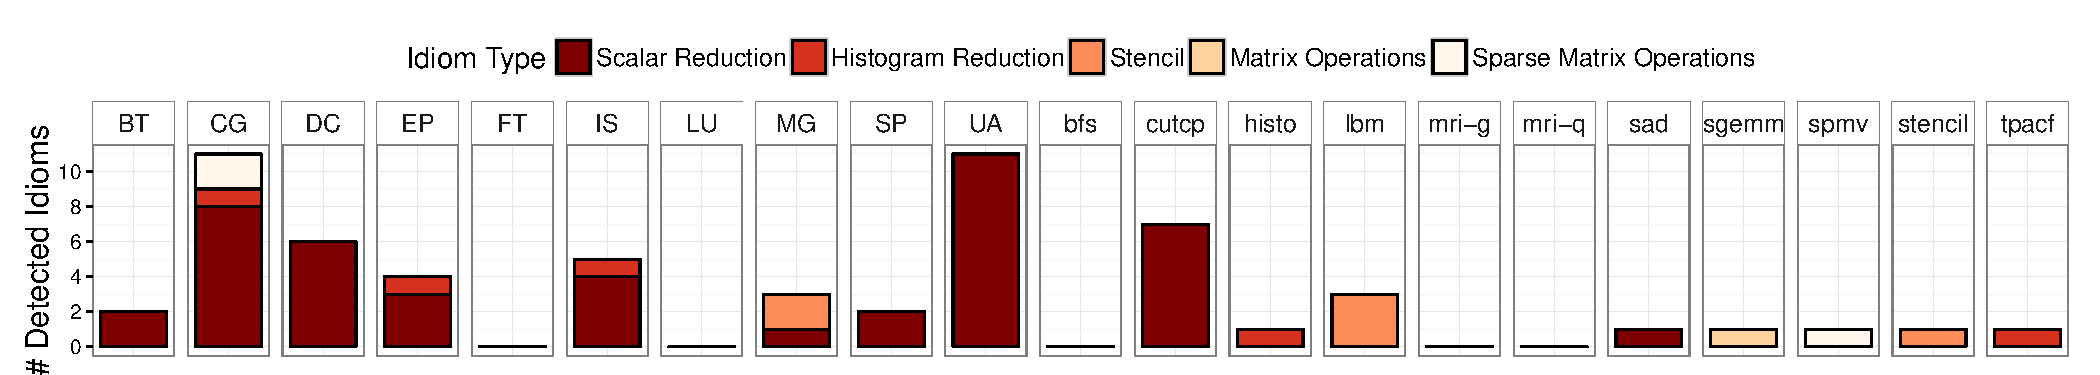
\includegraphics[width=\textwidth]{figures/asplosplots/detection.pdf}
  \caption{The different computational idioms found in all benchmarks.}
  \label{detection-figure}
\end{figure*}
\begin{figure*}[t]
  \centering
  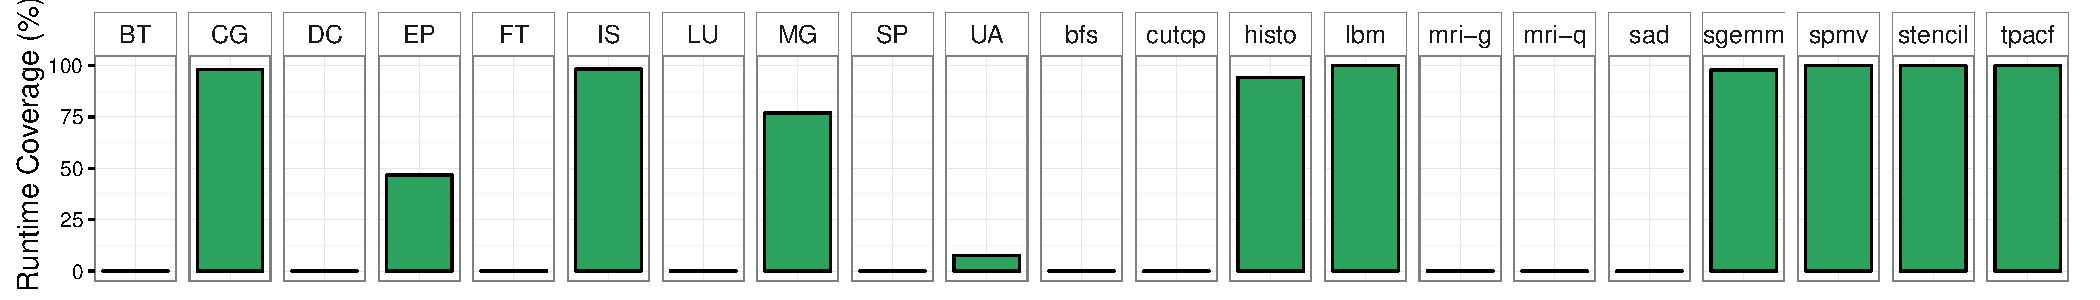
\includegraphics[width=\textwidth]{figures/asplosplots/coverage.pdf}
  \caption{Runtime coverage of the detected idioms in all benchmarks.}
  \label{coverage-figure}
  \vspace{0.5em}
\end{figure*}

\subsection{Idiom Detection}

    \autoref{tab:detection} shows the number of idioms found by our approach, Polly, and ICC.
    Polly finds 3 scalar reductions and 6 stencils while ICC which just considers  scalar reduction finds 28.
    Polly is unable to perform idiom specific optimizations on GEMM.
    Other approaches do not detect any histograms or sparse matrix operations, because such code involves indirect and thus non-affine memory accesses.
    This fundamentally contradicts assumptions that these tools rely on and is not merely an implementation artifact.
    Our IDL approach detects 60 idioms overall with the compile time cost shown in figure \autoref{tab:compiletimecost}.
    On average, the compilation time is increased by 82\%, which can be reduced further by optimizing the solver.

    \autoref{detection-figure} shows the different idioms detected across
    the  benchmarks. We detect both scalar
    and histogram reductions as well as stencils, dense matrix operations
    and sparse matrix-vector multiplication.
    While Polly and ICC are only capable of detecting simple scalar
    reductions we are able to detect histogram reductions, {\em e.g.} in
    the \emph{histo} benchmark as well.  For stencils, Polly detects two
    in \emph{lbm} and \emph{stencil} while our approach
    detects all the stencils in \emph{lbm}, \emph{stencil} and \emph{MG}.
    Unlike any existing approach, we detect sparse matrix-vector
    operations in {\emph CG} and {\emph spmv} as well as dense matrix
    operations in \emph{sgemm}. It is worth repeating, however, that both
    Polly and ICC are parallelizing compilers, not idiom recognition
    tools.

\begin{table}[t]
  \footnotesize
  \begin{tabular}{lP{1.16cm}P{1.16cm}P{1.16cm}P{1.163cm}P{1.163cm}}
  \toprule
  & Scalar\newline{}Reduction & Histogram\newline{}Reduction & Stencil & Matrix~Op. & Sparse\newline{}Matrix~Op.\\
  \midrule
  Polly &  3  &  --- &   5  &  --- & --- \\[0.25em]
  ICC   &  28 &  --- &  --- &  --- & --- \\[0.25em]
  IDL   &  45 &   5  &   6  &   1  &  3  \\
  \bottomrule
\end{tabular}

  \vspace{.1cm}
\caption{Idioms detected by IDL, ICC, Polly}
\label{tab:detection}
\vspace{-1em}
\end{table}

\subsection{Runtime Coverage}

    To determine if the detected idioms are actually important,
    \autoref{coverage-figure} shows the percentage of time spent in the detected
    computational idiom.
    This data shows that either the detected idioms have a low runtime
    contribution or they dominate almost the entire execution.
    \emph{EP} is the only exception where about 50\% of the runtime is spent
    inside a detected histogram reduction.
    We focus on the 10 programs which spend a significant amount of time in the
    detected idioms, as only these can reasonably expect a performance gain
    using our approach.

\subsection{Performance Results}

\addtolength{\tabcolsep}{-.3em}
\begin{table}[t]
  \scriptsize
  \begin{tabular}{lcccccccccccc}
  \toprule
  & \hspace{.631mm}BT\hspace{.631mm}
  & \hspace{.631mm}CG\hspace{.631mm}
  & \hspace{.631mm}DC\hspace{.631mm}
  & \hspace{.631mm}EP\hspace{.631mm}
  & \hspace{.631mm}FT\hspace{.631mm}
  & \hspace{.631mm}IS\hspace{.631mm}
  & \hspace{.631mm}LU\hspace{.631mm}
  & \hspace{.631mm}MG\hspace{.631mm}
  & \hspace{.631mm}SP\hspace{.631mm}
  & \hspace{.631mm}UA\hspace{.631mm}
  & \hspace{.631mm}bfs\hspace{.631mm}
  & \hspace{.631mm}cutcp\hspace{.631mm} \\
  \midrule
without IDL    & 1.9 & 0.5 & 1.0 & 0.3 & 0.6 & 0.3 & 1.9 & 0.8 & 1.6 & 2.7 & 0.4 & 0.4 \\[0.25em]
with IDL       & 4.0 & 0.8 & 1.6 & 0.6 & 1.2 & 0.5 & 3.9 & 4.5 & 3.2 & 7.3 & 0.5 & 0.6 \\[0.75em]
overhead in \% & 116 &  77 &  57 &  77 &  93 &  62 & 103 & 484 &  97 & 169 &  30 &  65 \\

  \bottomrule
\end{tabular}

\vspace{2em}

  \begin{tabular}{lccccccccc}
  \toprule
  & \hspace{0.530mm}histo\hspace{0.53mm}
  & \hspace{0.530mm}lbm\hspace{0.530mm}
  & \hspace{0.530mm}mri-g\hspace{0.530mm}
  & \hspace{0.530mm}mri-q\hspace{0.530mm}
  & \hspace{0.530mm}sad\hspace{0.530mm}
  & \hspace{0.530mm}sgemm\hspace{0.530mm}
  & \hspace{0.530mm}spmv\hspace{0.530mm}
  & \hspace{0.530mm}stencil\hspace{0.530mm}
  & \hspace{0.530mm}tpacf\hspace{0.530mm} \\
  \midrule
without IDL    & 0.2 & 0.3 & 0.2 & 0.2 & 0.4 & 0.6 & 0.3 & 0.2 & 0.2 \\[0.25em]
with IDL       & 0.2 & 0.6 & 0.4 & 0.3 & 0.6 & 0.7 & 0.7 & 0.2 & 0.4 \\[0.75em]
overhead in \% &  35 &  87 & 100 &  52 &  58 &  24 & 115 &  36 &  54 \\
  \bottomrule
\end{tabular}

  \vspace{.1cm}
\caption{Compile time cost in seconds}
\label{tab:compiletimecost}
\end{table}
\addtolength{\tabcolsep}{+.3em}

\paragraph{Speedup vs. Sequential}
\autoref{fig:speedup-figure} shows the end-to-end speedup obtained by accelerating idioms with heterogeneous APIs on a CPU, an integrated GPU, and an external GPU.
All results include data transfer overhead to and from the GPUs.
Here the best performing API is shown;
\autoref{tab:detailed-results} provides detailed results  for all APIs. 

\begin{figure*}[t]
  \centering
  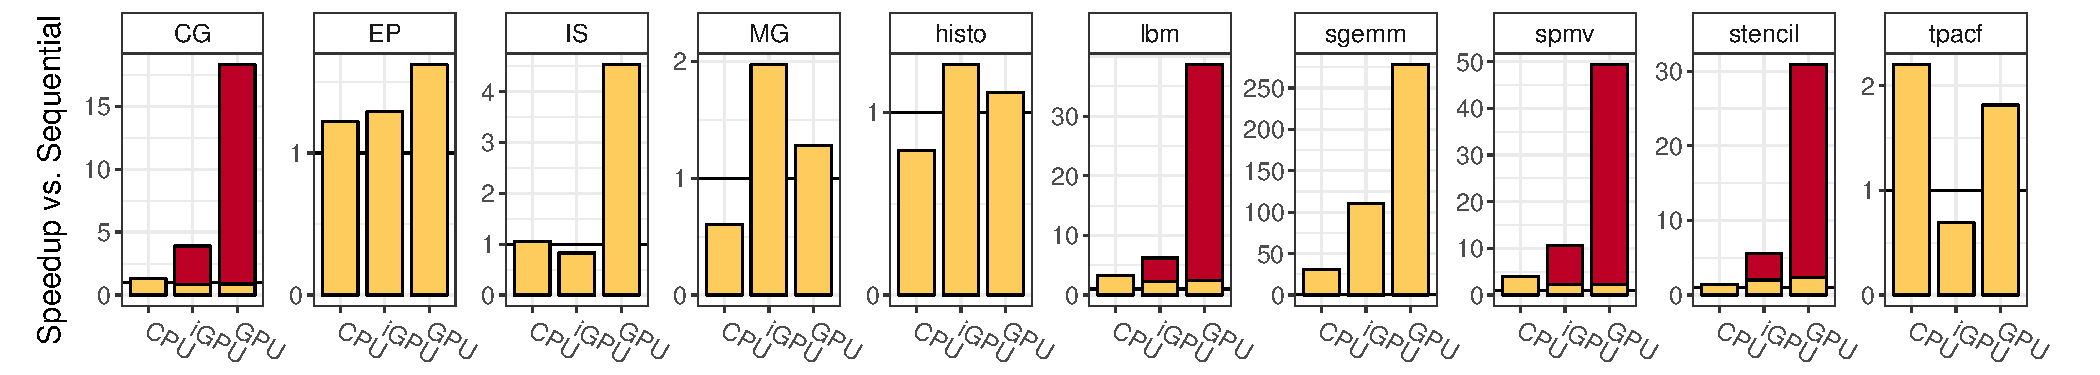
\includegraphics[width=\textwidth]{figures/asplosplots/speedup_vs_sequential_wide.pdf}
  \caption{Speedup compared to the sequential C program.
           Results for the best performing heterogeneous API on each device are shown.
           The red bars indicate a manual runtime optimization for avoiding unnecessary data transfers.}
  \label{fig:speedup-figure}
  \vspace{1.5em}
  \centering
  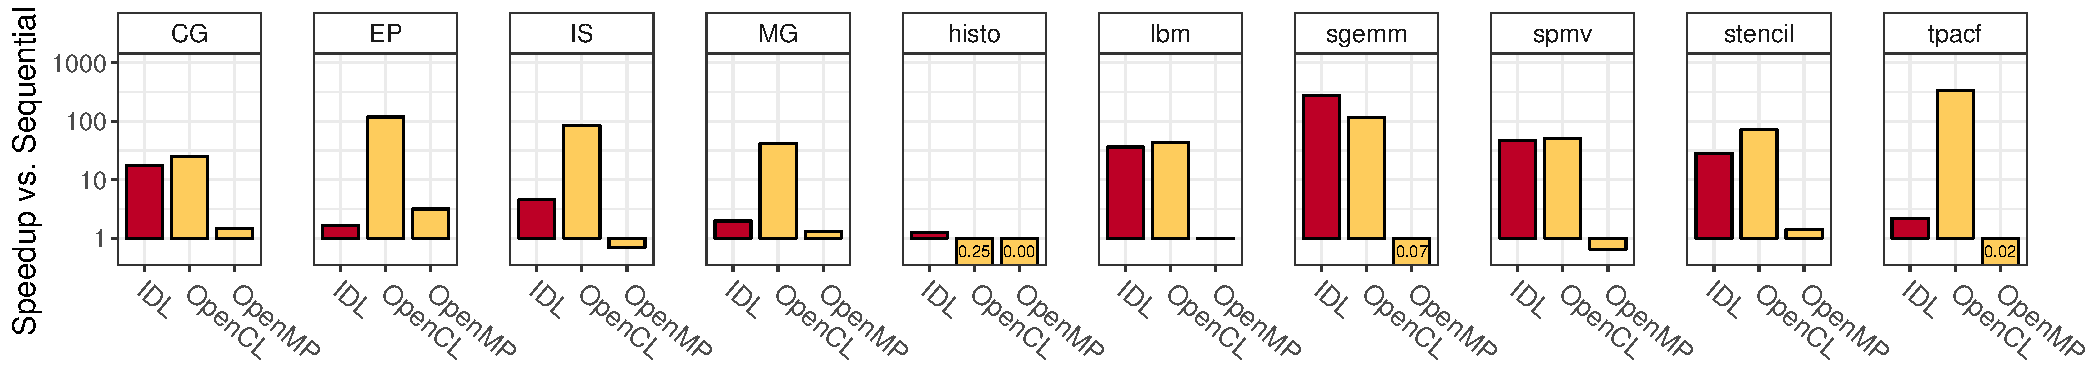
\includegraphics[width=\textwidth]{figures/asplosplots/comparison.pdf}
  \caption{Speedup of our constraints based approach (executed on the best hardware and highlighted in red) compared to handwritten parallel OpenCL (executed on the GPU) and OpenMP (executed on the CPU) implementations.}
  \label{fig:speedup-figure-2}
  \vspace{0.5em}
\end{figure*}

\newlength{\txtwd}
\newcommand{\msb}[1]{\settowidth{\txtwd}{#1}{\scriptsize\ttfamily\bfseries \hfill\tiny #1}}
\newcommand{\ms}[1]{\settowidth{\txtwd}{#1}{\scriptsize\ttfamily \hfill\tiny #1}}

\addtolength{\tabcolsep}{-.25em}
\begin{table*}
  \centering
  \scriptsize
  \begin{tabular}{l
                  P{0.146cm}
                  P{0.886cm} P{0.760cm} P{0.886cm} P{0.886cm} P{0.760cm} P{1.013cm}
                  P{0.146cm}
                  P{1.0cm} P{1.0cm} P{0.7cm} P{0.7cm} P{1.013cm}
                  P{0.146cm}
                  P{1.0cm} P{1.0cm} P{0.6cm} P{1.013cm}}
  \toprule
  & & \multicolumn{6}{c}{\bfseries\small CPU} & & \multicolumn{5}{c}{\bfseries\small iGPU} & & \multicolumn{4}{c}{\bfseries\small GPU} \\[0.5em]
  & & MKL & libSPMV & Halide & clBLAS & CLBlast & Lift & & clSPARSE & libSPMV & clBLAS & CLBlast & Lift & & cuSPARSE & libSPMV & cuBLAS & Lift \\
  \midrule
  {\footnotesize CG} &  & \msb{1504.21} & --- & --- & --- & --- & --- & & \msb{644.02} & --- & --- & --- & --- &  & \msb{113.51} & --- & --- & --- \\[0.5em]
  {\footnotesize EP} &  & --- & --- & --- & --- & --- &  \msb{32762.50} &  & --- & --- & --- & --- & \msb{30983.40}  & & --- & --- & --- & \msb{24680.70} \\[0.5em]
  {\footnotesize IS} &  & --- & --- & \msb{426.95} & ---  & --- & \ms{1765.61} &  &  --- & --- & --- & --- & \msb{547.28}  & & --- & --- & --- & \msb{99.95} \\[0.5em]
  {\footnotesize MG} &  & --- & --- & --- & --- & --- &  \msb{4699.63} &  & --- & --- & --- & --- & \msb{1439.58}  & & --- & --- & --- & \msb{2211.56} \\[0.5em]
  {\footnotesize histo} &  & --- & --- & --- & --- & --- &  \msb{27.42} &  & --- & --- & --- & --- & \msb{17.20}  & & --- & --- & --- & \msb{19.54} \\[0.5em]
  {\footnotesize lbm} &  & --- & --- & --- & --- & --- &  \msb{6457.93} &  & --- & --- & --- & --- & \msb{5335.09}  & & --- & --- & --- & \msb{590.60} \\[0.5em]
  {\footnotesize sgemm} &  & \msb{53.50} & --- & --- & \ms{1661.75} & \ms{660.44} & \ms{1339.15} &  & --- & --- & \msb{14.73} & \ms{19.03} & \ms{15.04}  & & --- & --- & \msb{5.99} & \ms{7.87} \\[0.5em]
  {\footnotesize spmv} &  & --- & \msb{218.17} & --- & --- & --- & --- & & --- &\msb{102.233} & --- & --- & --- & & --- &\msb{18.437} & --- &  ---\\[0.5em]
  {\footnotesize stencil} &  & --- & ---& \msb{5760.81} & --- & --- & \ms{21951.80} &  & --- & ---& --- & --- & \msb{2261.48} &  & --- & ---& --- & \msb{279.38} \\[0.5em]
  {\footnotesize tpacf} &  & --- & ---& --- & --- & --- & \msb{19276.40} &  & --- & ---& --- & --- & \msb{61111.90}  & & --- & ---& --- & \msb{23358.20} \\
  \bottomrule
\end{tabular}

  \vspace{.2cm}
\caption{Detailed performance results for each heterogeneous API used in milliseconds.
         Fastest implementations for each benchmark and target hardware are highlighted in bold.}
\label{tab:detailed-results}
\end{table*}
\addtolength{\tabcolsep}{+.25em}

For five benchmarks we obtain moderate speedups from 1.26$\times$ for \emph{histo} up to 4.5$\times$ for \emph{IS}.
All of these benchmarks (besides \emph{MG}) have a scalar or histogram reduction as their performance bottleneck and are, therefore, not computationally expensive.
Interestingly, we can see that different hardware is beneficial for different benchmarks:
for \emph{tpcaf}  the CPU is the best platform, beating the GPU  for which the data transfer time dominates;
for \emph{MG} and \emph{histo} the integrated GPU strikes the right balance between computational power while avoiding the movement of data to the external GPU;
and, finally, for \emph{EP} and \emph{IS} the data transfer to the GPU pays off exploiting the high GPU internal memory bandwidth.
These results emphasize the significance of heterogeneous code generation
flexibility.

For five of the benchmarks we achieve significantly higher performance gains, from 17$\times$ for \emph{CG} and up to over 275$\times$ for \emph{sgemm}.
These benchmarks are computationally expensive and the external GPU is always the fastest architecture by a considerable margin.

The red highlighting in the plot indicates an important runtime optimization:
redundant data transfers for the iterative \emph{CG}, \emph{lbm}, \emph{spmv} and \emph{stencil} benchmarks.
All of these benchmarks execute computations inside a for loop and do not require access to the data on the CPU between iterations.
We manually applied a straightforward lazy copying technique by flagging memory objects to avoid redundant transfers, similar to~\cite{jablin11automatic}.
As can be seen this runtime optimization is crucial for achieving high performance for these benchmarks.

\paragraph{API performance comparison}
\autoref{tab:detailed-results} provides a breakdown of the performance of each API on each program and platform.
Not all APIs
target all platforms, {\emph{e.g.} cuSPARSE only targets NVIDIA GPUs and in the
case of Halide, the current version that we have access to failed to generate
valid GPU code for any of the benchmarks we tried.
The best performing API is highlighted in bold in the table entries.
The \emph{spmv} benchmark uses an unusual sparse matrix format, so that we
implemented a custom library libSPMV for this benchmark.

On the multicore CPUs, the Intel MKL library gives the best linear algebra performance, outperforming the other libraries and Lift.
Halide achieves good performance for the NPB \emph{IS} and Parboil \emph{stencil} benchmarks on the CPU, outperforming Lift due to its more advanced vectorization capabilities.
In the programs where scalar reductions dominate, Lift performs well.
On the iGPU, clBLAS provides a better matrix-multiplication implementation than either CLBlast or Lift.
On the external GPUs, the libraries provide better linear algebra implementations, while Lift performs well on stencils and reductions.

\paragraph{Speedup vs. Parallel Handwritten Implementations}
\autoref{fig:speedup-figure-2} shows the performance of our approach compared to hand-written reference OpenMP and OpenCL implementations.
For some of the benchmarks, the parallel versions are significantly modified using different algorithms beyond the domain of automation.
We can see that for benchmarks where the handwritten implementation does not make algorithmic changes (\emph{CG}, \emph{histo}, \emph{lbm}, \emph{sgemm}, \emph{spmv}, \emph{stencil}), we achieve comparable -- or better -- performance.
For four benchmarks (\emph{EP}, \emph{IS}, \emph{MG}, and \emph{tpacf}) it is beneficial to parallelize the entire application -- which is beyond the scope of this paper. Future work will examine outer loop parallelism as an idiom to exploit.

For the \emph{sgemm} and \emph{stencil} benchmarks we improved the baseline implementation provided by the benchmarks as these had extremely poor performance.
A simple interchange of two loops improved performance by almost 20 times.

\paragraph{Summary}
We detect 60 idioms across the benchmark suites and are able to achieve significant performance improvements for those benchmarks where idioms dominate execution time by targeting different heterogeneous APIs.

\section{Related and Future Work}

\paragraph{Domain specific Languages}
DSLs have received much attention in recent years, ranging from SPIRAL \cite{ofenbeck13spiral},
a DSL for Fast Fourier Transforms, over Lift \cite{steuwer15rewrite, SteuwerRD17,HagedornSSGD18} to
UFL \cite{Alnaes:2014:UFL:2594412.2566630}, a DSL for partial
differential equations.  Stencils in particular have received much
attention \cite{Mullapudi:2015:PAO:2694344.2694364,HagedornSSGD18}, the best known of which is Halide
\cite{Ragan-Kelley2013Halide}. DSLs to exploit complex reductions are
less studied. In \cite{Reddy2016Reduction} they introduce a type of DSL via 
 annotations
that allow expression of complex reductions based on the
Platform-Neutral Compute Intermediate Language
\cite{baghdadi2015PENCIL}. In the case of matrix multiplication,
this is a well specified idiom supported by specific libraries
\cite{clblas,mkl,cublas}.

\paragraph{Generation of Performance Portable Code for Heterogeneous Hardware}
Recent research has highlighted the challenges of generating code that performs well on different heterogeneous hardware architectures.
PetaBricks~\cite{PhothilimthanaARA13} is one of the first languages to address this performance portability challenge by encoding algorithmic choices which are then empirically evaluated and automatically taken by the compiler.
Similarly \cite{MuralidharanRHG16} explores automatic selection of code variants using machine learning.
In a similar spirit, Lift~\cite{steuwer15rewrite} uses rewrite rules to explore optimization choices automatically.

\paragraph{Functional Code Generation Approaches}
There exist multiple functional approaches for generating code for heterogeneous hardware.
Accelerate is a Haskell embedded domain specific language aimed at generating efficient GPU code~\cite{chakravarty11accelerating,mcdonell13optimising}.
%Bergstrom and Reppy~\cite{BergstromR12} compile \textsc{Nesl}, which is a first-order dialect of ML supporting nested data-parallelism, to GPU code.
Recently, Nvidia introduced NOVA~\cite{collins14nova}, a new functional language targeted at code generation for GPUs, and Copperhead~\cite{catanzaro11copperhead}, a data parallel language embedded in Python.
%HiDP~\cite{zhang13hidp} is a hierarchical data parallel language which maps computations to OpenCL.
%All of these projects require programs to be rewritten in their functional language and rely on code analysis or hand-tuned versions of high-level algorithmic patterns to achieve high performance.
% 
%Halide~\cite{Ragan-Kelley2013Halide} is a domain specific approach that targets image processing pipelines.
%It separates the algorithmic description from optimization decisions.
% Our work is domain agnostic and takes a different approach.
% We systematically describe hardware paradigms as functional patterns instead of encoding specific optimizations which might not apply to future hardware generations.
% 
Delite~\cite{brown11heterogeneous,chafi11domain} is  a system that enables the creation of domain-specific languages using functional parallel patterns  and targets multi-core CPUs or GPUs.
% Alas, none of these approaches currently provides full performance portability, as they assume a fixed platform and the optimizations and implementations are targeted at a specific device.
%Spiral~\cite{pueschel05spiral} uses rewrite rules to optimize signal processing programs and was more recently adapted to linear algebra~\cite{Spampinato13LGen}.
 In contrast, to these approaches,
% we use rewrite rules and low-level hardware patterns to produce high-performan%ce code in a portable way and
we  require no rewriting of legacy programs.

\paragraph{Idiom Detection}
Idiom based optimization \cite{Pinter:1994:POP:177492.177494} has
fallen out of fashion, with more systematic approaches
based on SSA \cite{lattner2004llvm} and polyhedral representations
\cite{benabderrahmane2010polyhedral}.
They were largely based on syntactic pattern matching and not robust in the presence of complex control and dataflow.
More recently, \cite{Andion2015Compilation} describes a compiler based
parallelization approach for heterogeneous computing, based on
an idiomatic intermediate representation called KIR.  
 It is not clear how such an approach would work on general
C/C++ programs.

\paragraph{Stencils}
Stencil detection has been driven by the introduction of DSLs such as
Halide.  Helium \cite{Mendis2015Helium} tackles the challenging task
of detecting stencils in binary code. It relies
on dynamic analysis and cannot easily be extended to
other idioms.
Another closely related paper is \cite{Kamil2016Verified}, which detects stencils in FORTRAN by the
verified lifting of code segments to a representation that can be
mapped to Halide DSL.  It uses syntax guided synthesis to verify
translation with added constrains to ensure that it can be mapped to
Halide.
It however requires nested loops  without conditionals in well behaved FORTRAN
and in some cases requires user annotations.

\paragraph{Reductions}
Discovering and exploiting scalar reductions in programs has been
studied for many years based on dependence analysis and idiom detection
 \cite{fisher1994parallelizing,pottenger1995idiom,suganuma1996detection}.
Alongside this data dependence based approach, there has also been a
 large body of work exploring mapping of reductions in a
 polyhedral setting \cite{jouvelot1989unified,redon1994scheduling}
 The treatment of
more general reduction operations has received  less attention.
Work has focused on exploitation rather than discovery
\cite{Gutierrez:2000,gutierrez2003optimization,gutierrez2008analytical}, examining trade-offs in implementation \cite{yu2006adaptive}
 or exploitation of novel hardware \cite{ravi2010compiler,Huo2011HiPC}.
Recent work \cite{ginsbach2017discovery} shows that more complex reductions can be 
detected, but this is tied to  an  ad~hoc non-portable code generation phase. 

\paragraph{Polyhedral Approaches}
Polyhedral compilers \cite{Baskaran:2010:ACC:2175462.2175482,Verdoolaege:2013:PPC:2400682.2400713} perform advanced loop optimizations and have been used for the generation of fast GPU kernels.
More recently, extensions to the polyhedral framework have been proposed, allowing it to capture reduction computations \cite{chi1997optimizing, gupta2006simplifying, stock2014framework}.
Such efforts are described in \cite{Doerfert2015Polly}, but they are fragile in the presence of non static control flow.

\paragraph{Future Work}
Although idioms can be described concisely with IDL, we currently
have to implement a separate translation scheme for each API. While
much of the translation code is common, it would be preferable to have
an API description language similar to IDL that allows automatic
generation of API translators. This would allow rapid evaluation of
different APIs for the same idiom.

As the number of APIs and idioms grows, a profitability heuristic
will be needed to determine the best API to use for each
program and platform.  Machine learning approaches are an obvious
starting point as they easily adapt to changing targets.

This paper restricts its attention to five common idioms. Other idioms
such as graph processing can also be described. Given that IDL works on
the compiler IR, loop and function parallelism can also be
described as idioms.
In those cases where user codes do not quite match the platform API
and associated idioms, we can apply
program transformations to refactor or rejuvenate code to fit.

To be a robust approach to heterogeneous programming, we need to ensure correctness.
Syntax guided synthesis is a promising means of verifying the idiom translation.

It would be interesting  to see to whether our approach  could be used for binary optimization or  applied to 
heavily optimized and  complex code bases.
Another  research direction  is investigating explicitly parallel legacy codes.

\section{Conclusion}

    This paper develops a compiler based approach that automatically
    detects a wide class of idioms supported by libraries or domain
    specific languages for heterogeneous processors. This approach is
    based on a constraint based description language that identifies
    program subsets that adhere to idiom specifications.  Once
    detected, the idioms are mechanically translated into API calls to
    external libraries or code generated by DSL compilers.

    This approach is robust and was evaluated on C/C++ versions of two well
    known benchmark suites: NAS and Parboil. We detected more stencils,
    sparse matrix operations and generalized reductions and histograms than
    existing approaches and generated fast code.

    Future work will extend the constraint formulation to consider other common
    idioms.
    As the number of idioms detected and of implementations available grows, a
    smart profitability analysis will be needed and is the subject of future
    work.

